\section{Triển khai và Thực nghiệm}

\subsection{Ứng dụng DDD}

\begin{frame}{Cấu trúc A/B Test}
	\begin{table}
		\begin{tabular}{|l|l|l|}
			\hline
			Thực thể                    & Khuôn mẫu    & Giải thích                           \\ \hline
			\multirow{2}{*}{Product}    & Entity       & Product có id định danh riêng        \\ \cline{2-3}
			                            & Aggregate    & Product là tổng hợp của các Layers   \\ \hline
			\multirow{2}{*}{Layer}      & Entity       & Layer có id định danh riêng          \\ \cline{2-3}
			                            & Aggregate    & Layer là tổng hợp của các Experiment \\ \hline
			\multirow{2}{*}{Experiment} & Entity       & Experiment có id định danh riêng     \\ \cline{2-3}
			                            & Aggregate    & Experiment có nhiều Test Group       \\ \hline
			\multirow{2}{*}{Test Group} & Entity       & Test Group có id định danh riêng     \\ \cline{2-3}
			                            & Aggregate    & Test Group gồm nhiều Parameter       \\ \hline
			Parameter                   & Value object & Parameter không có định danh         \\ \hline
		\end{tabular}
	\end{table}
\end{frame}

\begin{frame}{Hệ thống Backend}
	\begin{table}
		\begin{tabular}{|l|l|p{7cm}|}
			\hline
			Thực thể & Khuôn mẫu                 & Giải thích                                                                             \\ \hline
			Service  & \multirow{2}{*}{Services} & Service chịu trách nghiệm điều phối hoạt động giữa các tầng thông qua phương thức HTTP \\ \cline{1-1} \cline{3-3}
			Storage  &                           & Storage chịu trách nghiệm tổng hợp các Entity từ tầng Database                         \\ \hline
			Database & Repository                & Database là tầng trung gian giữa các tầng khác và tầng cơ sở dữ liệu (Redis)           \\ \hline
			Types    & Aggregate                 & Types là nơi tổng hợp các Entities và các Value Object                                 \\ \hline
		\end{tabular}
	\end{table}
\end{frame}

\subsection{Thực nghiệm}

% \begin{frame}{Hiển thị tất cả Product}
% 	\begin{figure}
% 		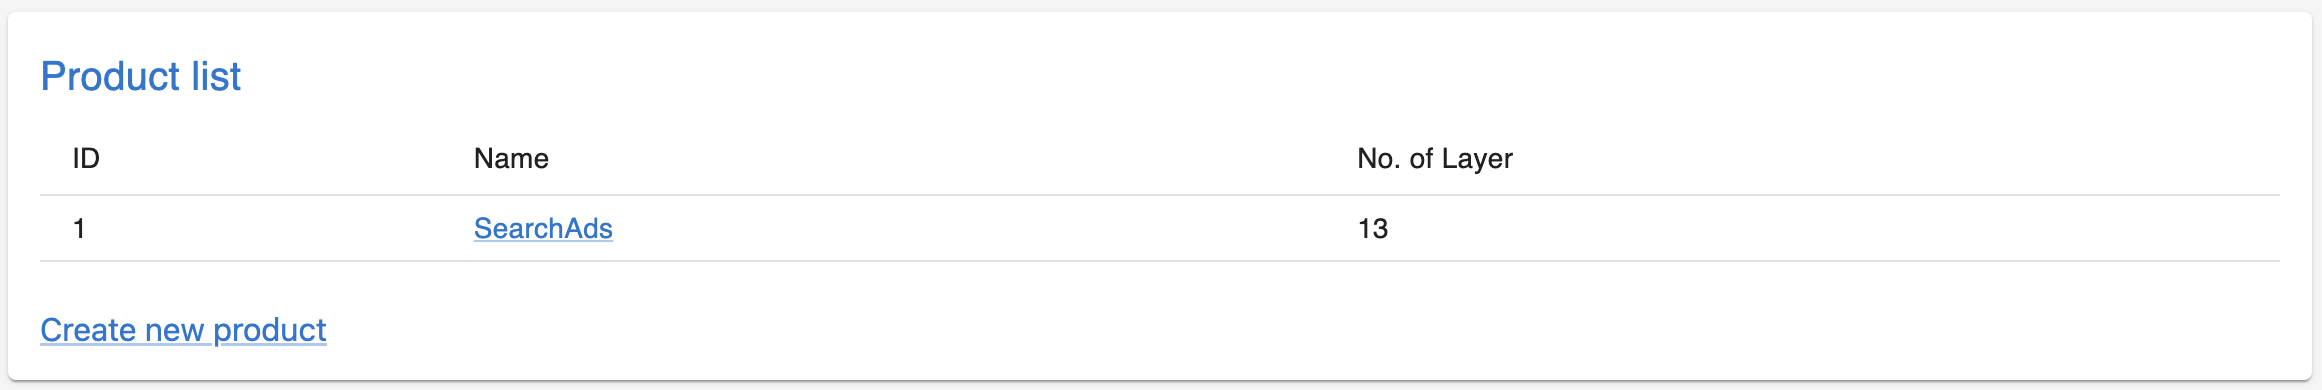
\includegraphics[width = 1\textwidth]{all-products}
% 	\end{figure}
% \end{frame}
%
% \begin{frame}{Hiển thị thông tin của một Product}
% 	\begin{figure}
% 		\centering
% 		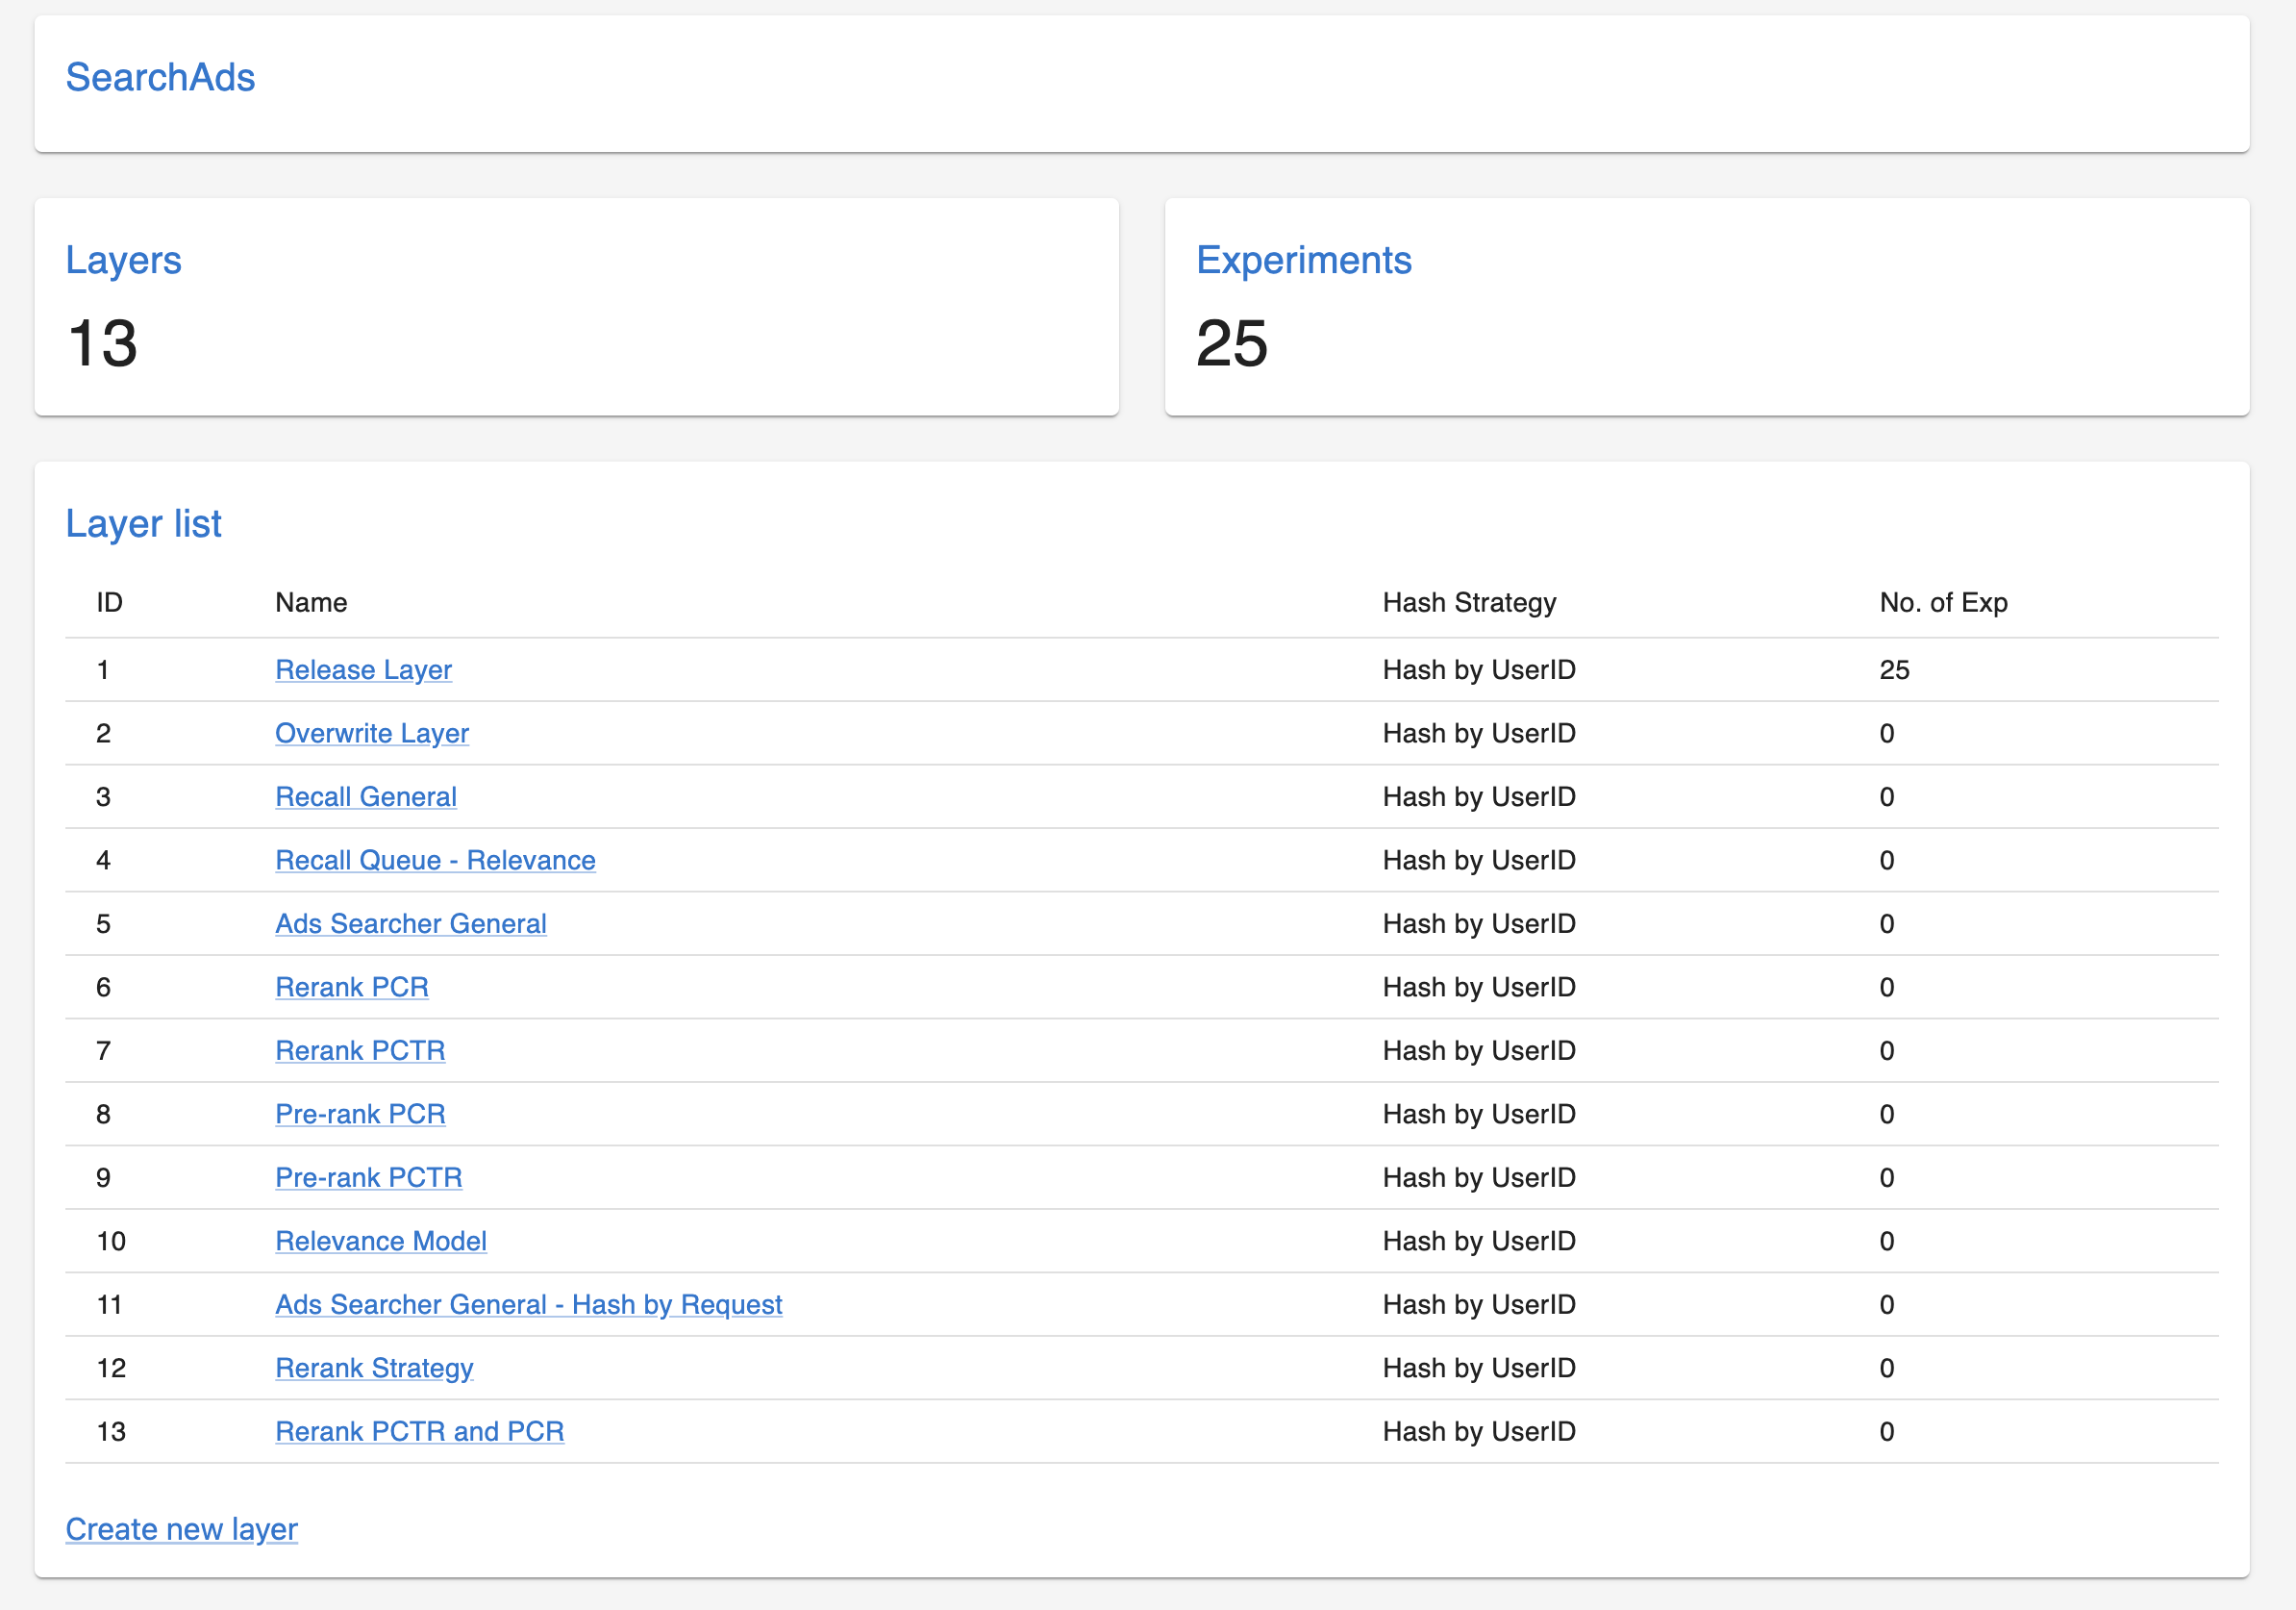
\includegraphics[width = 1\textwidth]{one-product}
% 	\end{figure}
% \end{frame}
%
% \begin{frame}{Hiển thị thông tin của một Layer}
% 	\begin{figure}
% 		\centering
% 		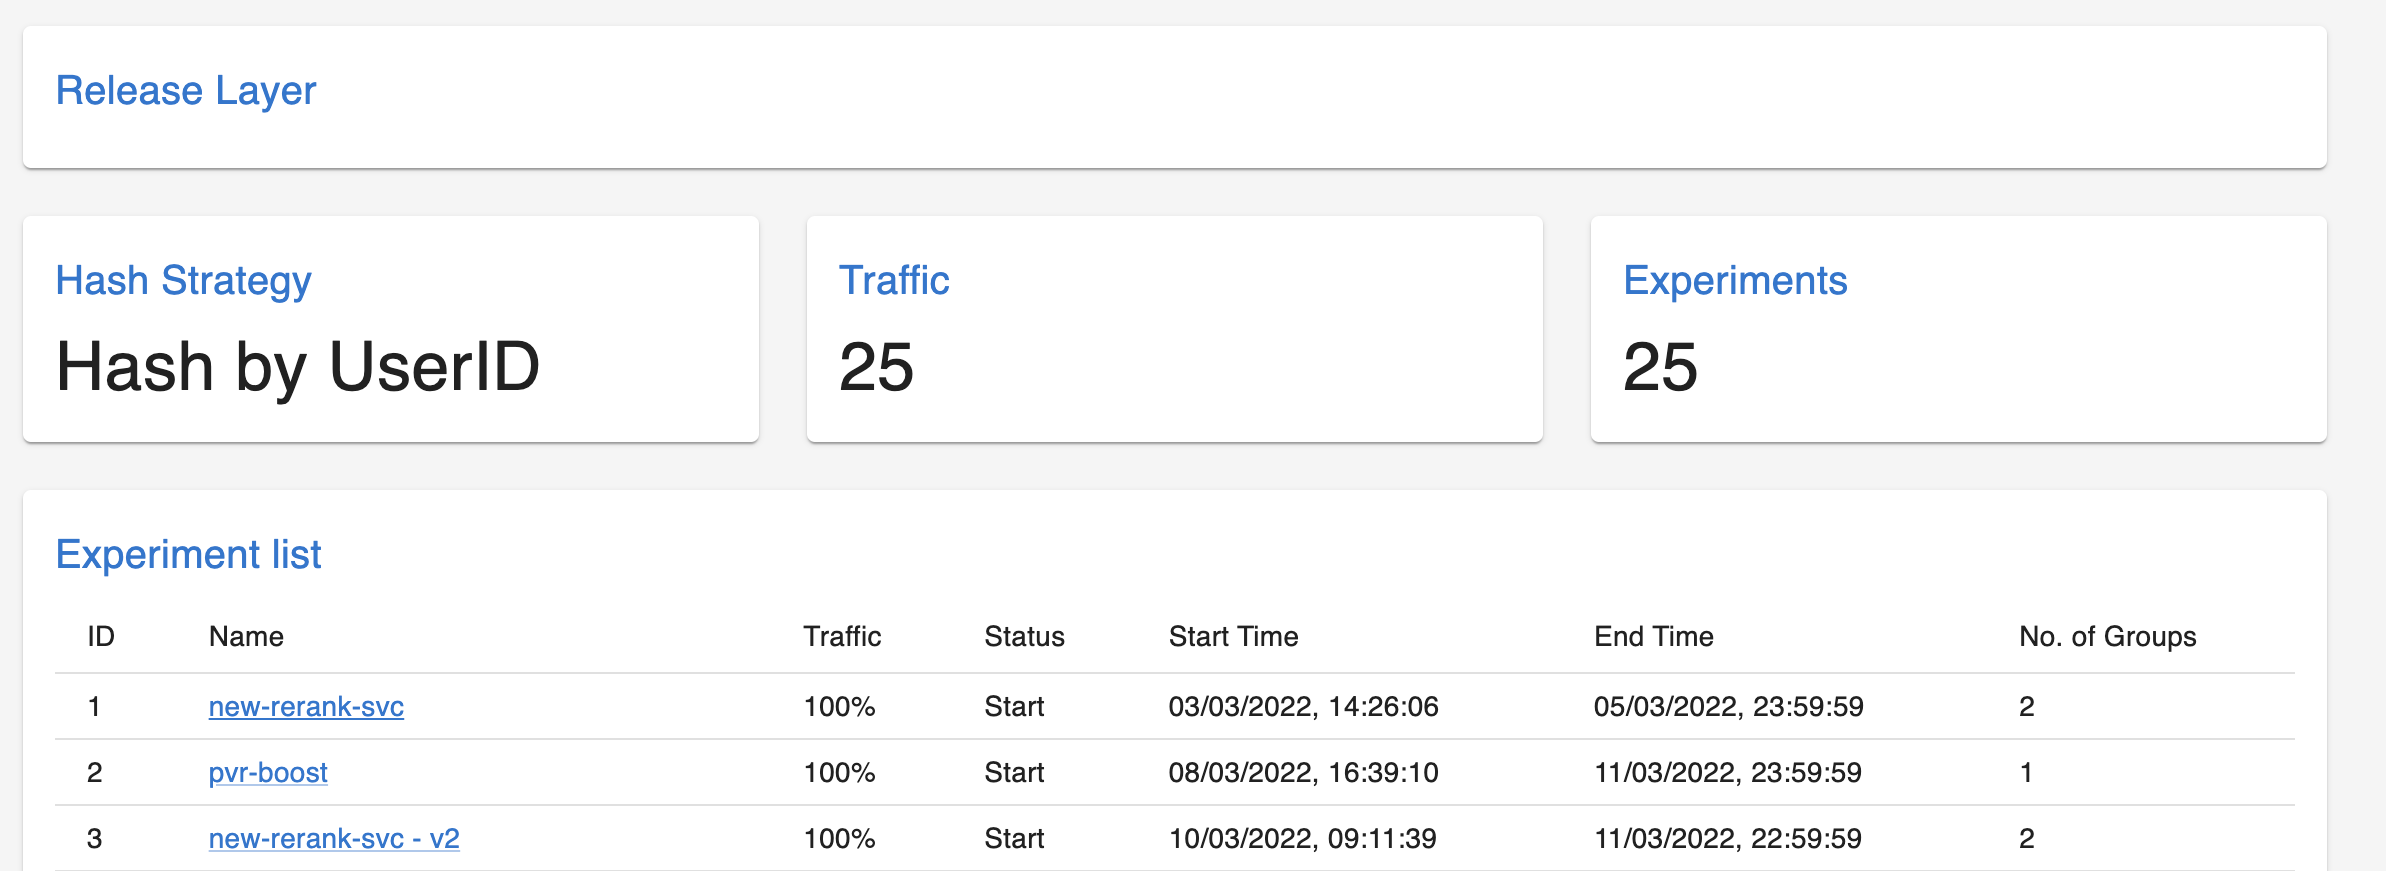
\includegraphics[width = 1\textwidth]{one-layer}
% 	\end{figure}
% \end{frame}

\begin{frame}{Sau khi khởi tạo A/B Test}
	\begin{figure}
		\centering
		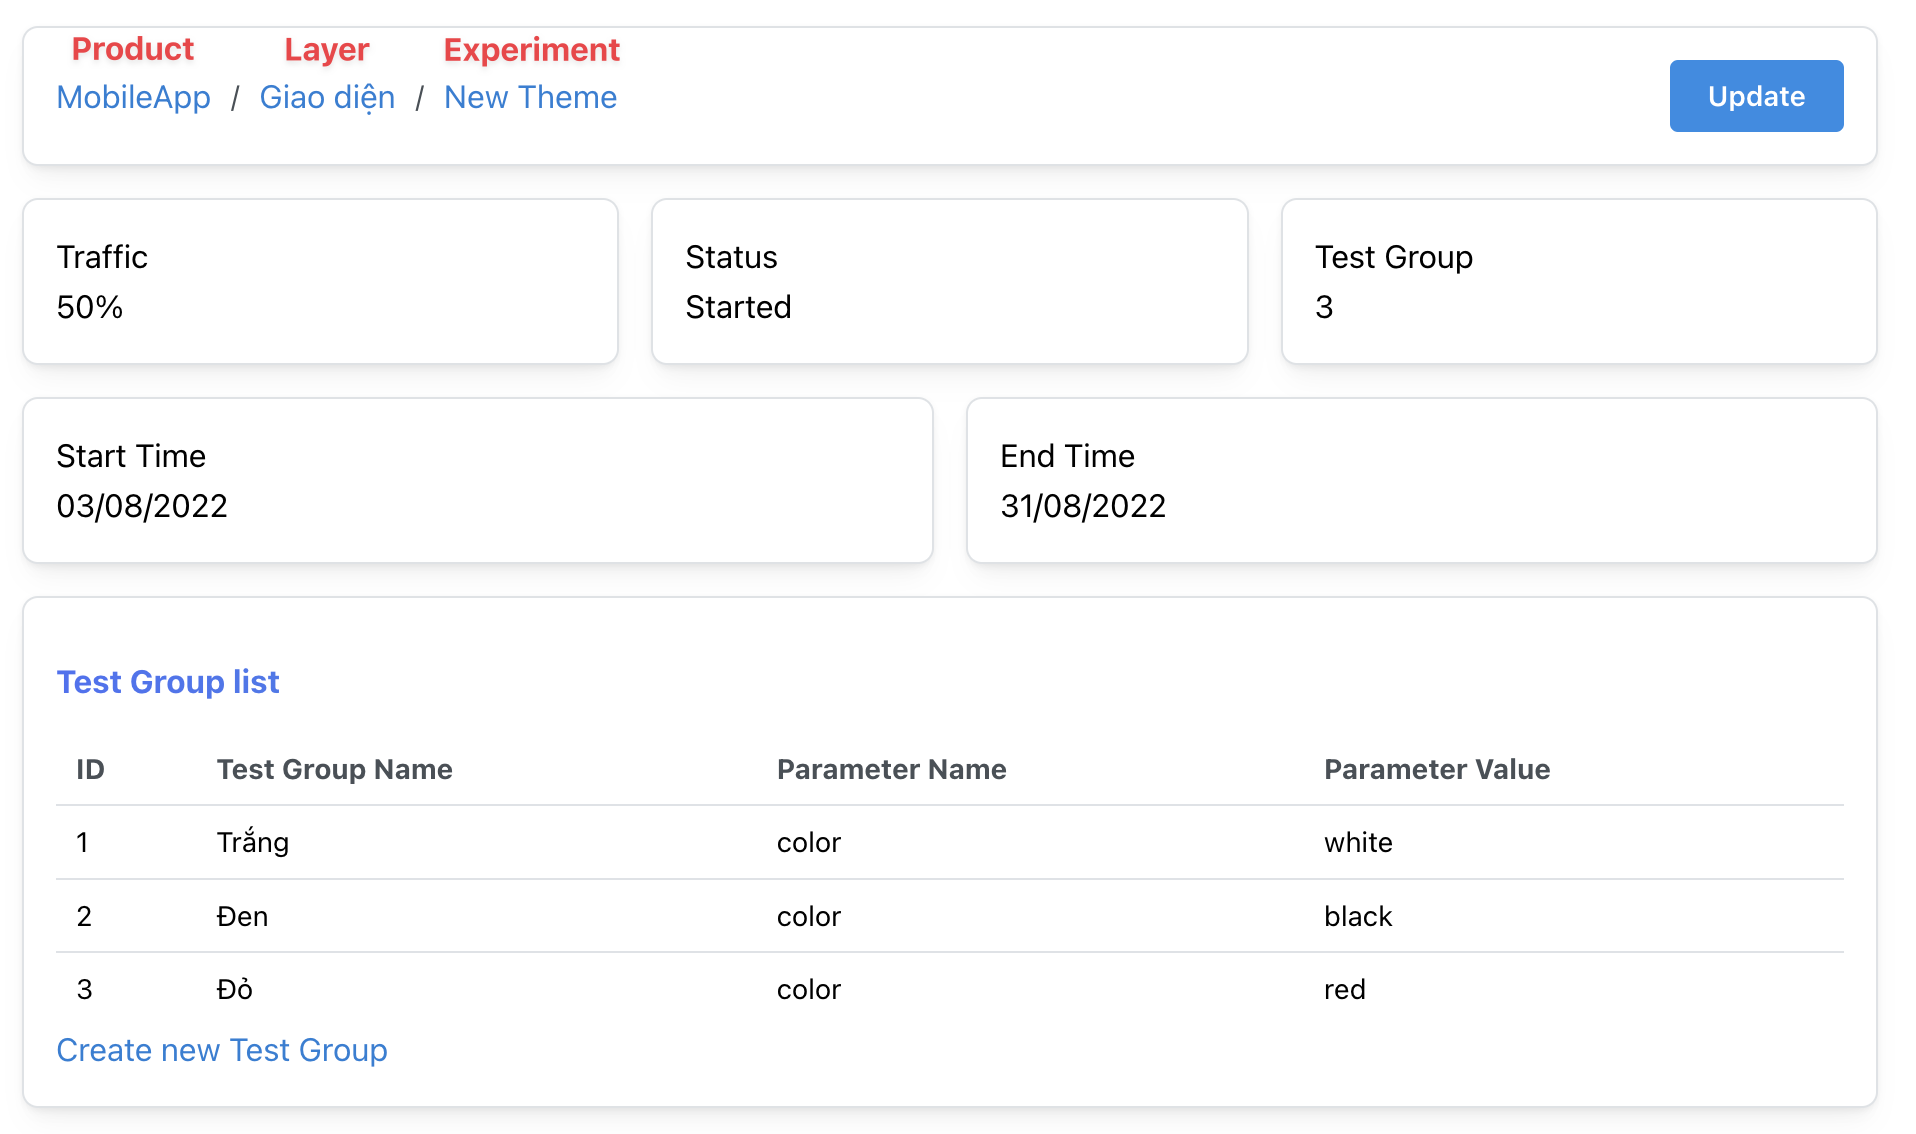
\includegraphics[width = 1\textwidth]{all-test-group}
	\end{figure}
\end{frame}

\begin{frame}{Kết quả thí nghiệm}
	\begin{columns}
		% Column 1
		\begin{column}{0.5\textwidth}
			\begin{figure}
				\centering
				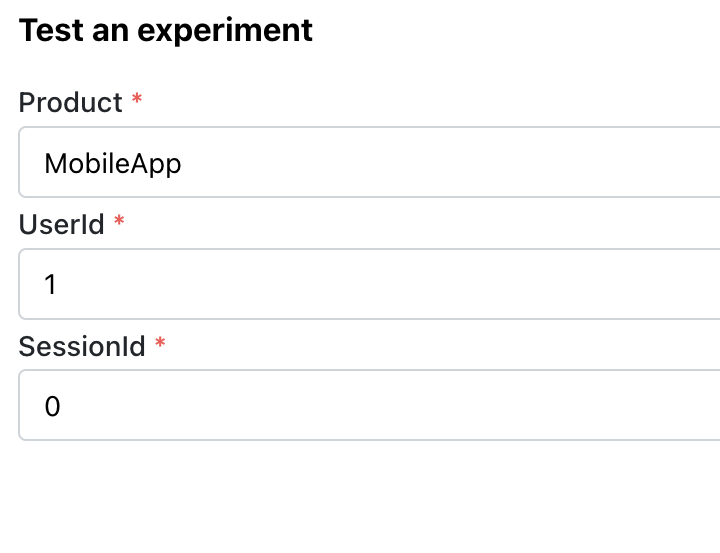
\includegraphics[height = 1\textwidth,width = 1\textwidth]{ab-experiment}
			\end{figure}
		\end{column}
		% Column 2
		\begin{column}{0.5\textwidth}
			\begin{figure}
				\centering
				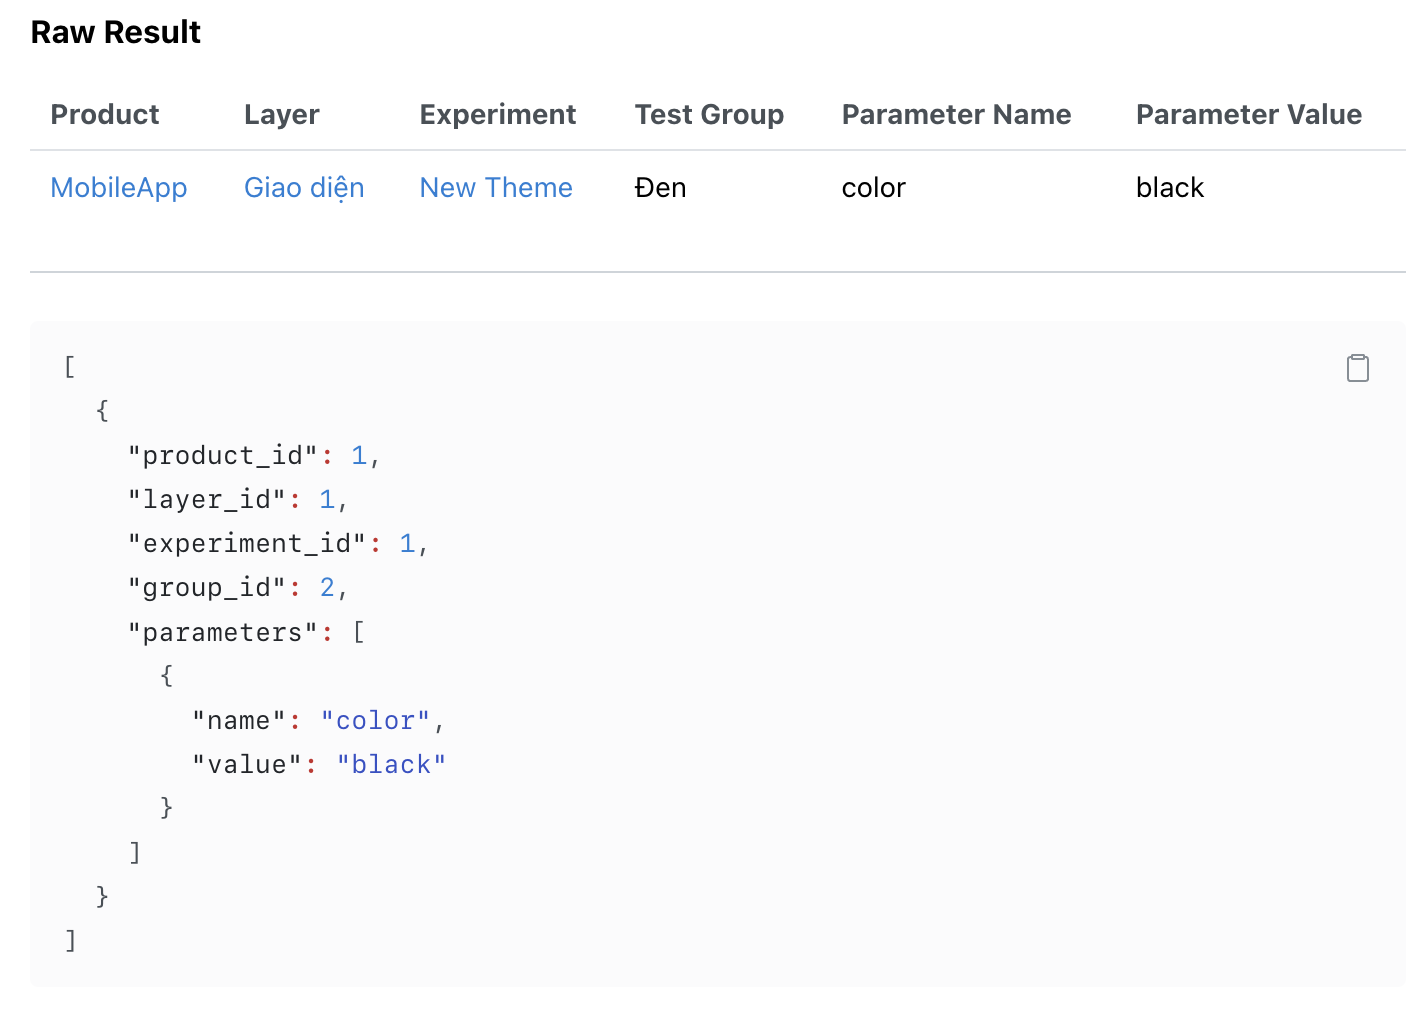
\includegraphics[height = 1\textwidth,width = 1\textwidth]{experiment-result}
			\end{figure}
		\end{column}
	\end{columns}
\end{frame}
